\documentclass[11pt,a4paper]{article}
\usepackage[utf8]{inputenc}
\usepackage[T1]{fontenc}
\usepackage{geometry}
\usepackage{hyperref}
\usepackage{listings}
\usepackage{xcolor}
\usepackage{booktabs}
\usepackage{parskip}
\usepackage{enumitem}
\usepackage{tikz}
\usetikzlibrary{shapes.geometric, arrows.meta, positioning, fit, calc, decorations.pathreplacing}

\geometry{margin=1in}
\hypersetup{colorlinks=true, linkcolor=blue, urlcolor=blue}

\lstdefinestyle{mystyle}{
    backgroundcolor={\color{gray!8}},
    basicstyle=\ttfamily\footnotesize,
    breaklines=true,
    frame=single,
    framesep=4pt,
}
\lstset{style=mystyle}

\title{\textbf{RimRun: Address Field \& Map Preview} \\ \large How Typing Moves the Map (Tutorial)}
\author{Technical documentation}
\date{\today}

\begin{document}
\maketitle
\tableofcontents
\newpage

%==============================================================================
\section{What Problem This Solves}
%==============================================================================

On the \textbf{Add court} screen (\texttt{app/(app)/court/add.tsx}), the user can:
\begin{enumerate}[noitemsep]
    \item Place the court using only the \textbf{map} (crosshair = center of the map), or
    \item Type an \textbf{address} so latitude/longitude come from \textbf{geocoding} (turning text into coordinates), not from the map or GPS.
\end{enumerate}

If the user types an address, you want the \textbf{map to visually follow} that address so they can confirm the right area---without spamming the geocoder on every keystroke or showing error alerts while they are still typing.

This document explains \textbf{debouncing}, \textbf{stale async requests}, \textbf{React refs vs state}, and \textbf{how Expo's \texttt{geocodeAsync}} fits in.

\begin{figure}[h]
\centering
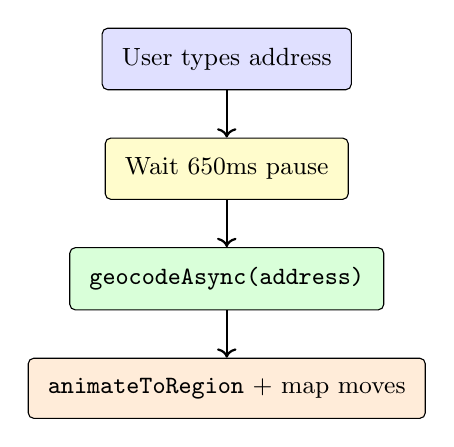
\begin{tikzpicture}[node distance=0.6cm, box/.style={rectangle, draw, rounded corners=2pt, align=center, font=\small, inner sep=0.25cm}]
  \node[box, fill=blue!12] (t) {User types address};
  \node[box, fill=yellow!20, below=of t] (w) {Wait 650ms pause};
  \node[box, fill=green!15, below=of w] (g) {\texttt{geocodeAsync(address)}};
  \node[box, fill=orange!15, below=of g] (m) {\texttt{animateToRegion} + map moves};
  \draw[->, thick] (t) -- (w);
  \draw[->, thick] (w) -- (g);
  \draw[->, thick] (g) -- (m);
\end{tikzpicture}
\caption{Preview pipeline: pause → geocode → pan map (silent on failure).}
\end{figure}

%==============================================================================
\section{Prerequisites: Concepts in Plain English}
%==============================================================================

\subsection{Geocoding vs.\ reverse geocoding}

\paragraph{Forward geocoding (what we use here.)}
You have a \textbf{string} like ``123 Main St, Austin, TX'' and a service returns \textbf{latitude} and \textbf{longitude}. Expo exposes this as \texttt{Location.geocodeAsync(address)}.

\paragraph{Reverse geocoding.}
You have coordinates and want a human address. That is \texttt{Location.reverseGeocodeAsync}---not used for this preview.

\subsection{Why not geocode on every keypress?}

Each call may hit Apple/Google services and can be \textbf{rate-limited} or slow. Typing ``Main Street'' would trigger 10+ requests if you geocoded after every character. So we wait until the user \textbf{pauses} (\textbf{debounce}).

\subsection{Debouncing (the intuition)}

Imagine a \textbf{resetting timer}: every time the user types, you cancel the old timer and start a new \textbf{650ms} countdown. Only when the timer fires without being reset do you run geocode.

\begin{figure}[h]
\centering
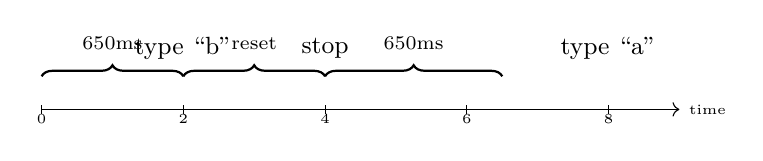
\begin{tikzpicture}[x=0.9cm, y=0.7cm]
  \draw[->] (0,0) -- (9,0) node[right, font=\tiny] {time};
  \foreach \x in {0,2,4,6,8} \draw (\x,-0.08) -- (\x,0.08) node[below, font=\tiny] {\x};
  \draw[decorate, decoration={brace, amplitude=4pt}, thick] (0,0.6) -- (2,0.6) node[midway, above=6pt, font=\scriptsize] {650ms};
  \draw[decorate, decoration={brace, amplitude=4pt}, thick] (2,0.6) -- (4,0.6) node[midway, above=6pt, font=\scriptsize] {reset};
  \draw[decorate, decoration={brace, amplitude=4pt}, thick] (4,0.6) -- (6.5,0.6) node[midway, above=6pt, font=\scriptsize] {650ms};
  \node[font=\small] at (8,1.1) {type ``a''};
  \node[font=\small] at (2,1.1) {type ``b''};
  \node[font=\small] at (4,1.1) {stop};
\end{tikzpicture}
\caption{Each keystroke resets the debounce window; geocode runs only after quiet time.}
\end{figure}

\subsection{Stale async results (race conditions)}

Typing is fast; geocoding is slow. Request A for ``Austin'' might return \emph{after} a newer request B for ``Austin TX.'' If you always applied the last result to arrive, you could be wrong. You need to \textbf{drop} results that are no longer current.

RimRun uses a \textbf{generation counter} (monotonic integer): before each request starts, increment \texttt{addressPreviewGen}. When the response arrives, compare the \textbf{generation at start} with the \textbf{current} value; if they differ, discard the result.

\begin{figure}[h]
\centering
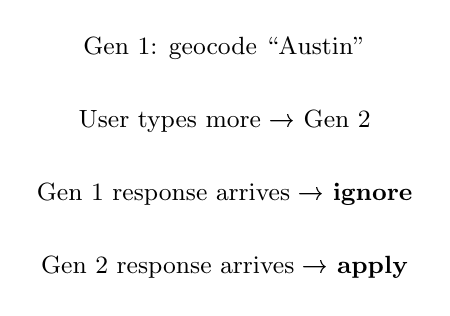
\begin{tikzpicture}[node distance=0.4cm, font=\small]
  \node (a) {Gen 1: geocode ``Austin''};
  \node[below=of a] (b) {User types more → Gen 2};
  \node[below=of b] (c) {Gen 1 response arrives → \textbf{ignore}};
  \node[below=of c] (d) {Gen 2 response arrives → \textbf{apply}};
\end{tikzpicture}
\caption{Generation counter: only the latest intended request wins.}
\end{figure}

\subsection{React: \texttt{useRef} vs \texttt{useState}}

\begin{itemize}[noitemsep]
    \item \textbf{\texttt{useState}}: changing it \textbf{re-renders} the component. Good for UI that must reflect the value (e.g.\ text field).
    \item \textbf{\texttt{useRef}}: mutable \texttt{.current} without forcing a re-render. Good for: \textbf{storing a stable map region for “home GPS,”} \textbf{counters}, and \textbf{flags} that should not trigger extra renders.
\end{itemize}

The map's visible region is \textbf{also} in \texttt{useState} (\texttt{region}) so React can reconcile when needed; ``home'' GPS is duplicated in \texttt{gpsRegionRef} so we can snap back without deriving it from the geocoded preview.

%==============================================================================
\section{Constants in Code}
%==============================================================================

\begin{center}
\begin{tabular}{@{}ll@{}}
\toprule
\textbf{Constant} & \textbf{Role} \\
\midrule
\texttt{MIN\_ADDRESS\_PREVIEW\_CHARS = 4} & Do not geocode until at least \textbf{4} non-space characters after \texttt{trim}. Avoids useless queries for ``St'' or ``12.'' \\
\texttt{ADDRESS\_DEBOUNCE\_MS = 650} & Milliseconds of quiet time after last change before running preview geocode. \\
\texttt{ZOOM\_DELTA = 0.008} & Latitude/longitude span of the map window (how zoomed in the preview is). \\
\bottomrule
\end{tabular}
\end{center}

\textbf{Why 4 characters?} A tradeoff: shorter thresholds fire more often; longer thresholds feel sluggish. Four is a simple heuristic.

\textbf{Why 650ms?} Long enough to avoid firing on every syllable; short enough to feel responsive. Alternatives: 300ms (more aggressive) or 1000ms (calmer).

%==============================================================================
\section{Refs Used in the Preview}
%==============================================================================

\begin{description}[style=nextline, leftmargin=1.5cm]
    \item[\texttt{gpsRegionRef}] Holds the last \textbf{GPS / initial} map region (device location, or fallback San Francisco, or updated when you tap \textbf{My location}). When the user \textbf{clears} the address field, the map animates back to \textbf{this} region---not to the last geocoded preview.

    \item[\texttt{addressPreviewGen}] Integer. Incremented before each \texttt{geocodeAsync} in the preview effect. After the async call returns, if \texttt{myGen !== addressPreviewGen.current}, the result is \textbf{stale}.

    \item[\texttt{hadAddressContentRef}] Boolean semantics: \textbf{true} once the user has entered text in the address field. When the field becomes \textbf{empty} again, if this was \textbf{true}, we restore \texttt{gpsRegionRef} (snap back). On first mount \texttt{address} is empty but we did \textbf{not} have content before, so we \textbf{do not} animate the map (avoids fighting the initial GPS load).

\end{description}

\begin{figure}[h]
\centering
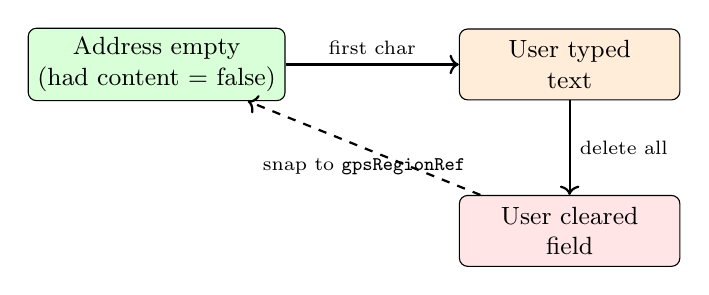
\begin{tikzpicture}[
  state/.style={rectangle, draw, rounded corners=3pt, minimum width=2.8cm, minimum height=0.9cm, align=center, font=\small},
  arr/.style={->, thick}
]
  \node[state, fill=green!15] (empty) {Address empty\\(had content = false)};
  \node[state, fill=orange!15, right=2.2cm of empty] (typing) {User typed\\text};
  \node[state, fill=red!10, below=1.2cm of typing] (cleared) {User cleared\\field};
  \draw[arr] (empty) -- node[above, font=\scriptsize] {first char} (typing);
  \draw[arr] (typing) -- node[right, font=\scriptsize] {delete all} (cleared);
  \draw[arr, dashed] (cleared) -- node[below, font=\scriptsize] {snap to \texttt{gpsRegionRef}} (empty);
\end{tikzpicture}
\caption{When to restore GPS: only after the user had typed something, then cleared.}
\end{figure}

%==============================================================================
\section{The \texttt{useEffect} on \texttt{address}}
%==============================================================================

The effect depends only on \texttt{[address]}---not on \texttt{region}. If \texttt{region} were in the dependency array, the effect would re-run after \texttt{setRegion} from the geocode, causing a \textbf{loop} or repeated geocodes.

\paragraph{Cleanup:} \texttt{return () => clearTimeout(timer)} cancels the pending debounce when the user types again before 650ms, or when the component unmounts.

\paragraph{Empty branch:} If \texttt{trimmed.length === 0}, reset \texttt{hadAddressContentRef} to false; \textbf{if} it was true before, animate to \texttt{gpsRegionRef}.

\paragraph{Non-empty branch:} Set \texttt{hadAddressContentRef} true. If length $<$ \texttt{MIN\_ADDRESS\_PREVIEW\_CHARS}, return (no timer yet).

\paragraph{Debounce branch:} After timeout, increment generation, \texttt{geocodeAsync}, on success \texttt{animateToRegion} and \texttt{setRegion}. Errors are \textbf{silent} (preview should not spam alerts).

%==============================================================================
\section{Preview vs.\ Save (\texttt{resolveCourtCoordinates})}
%==============================================================================

Both paths use \texttt{Location.geocodeAsync} when the address is non-empty.

\begin{center}
\begin{tabular}{@{}p{4.2cm}p{4.2cm}p{4.2cm}@{}}
\toprule
\textbf{Aspect} & \textbf{Preview (while typing)} & \textbf{Submit (\texttt{handleSubmit})} \\
\midrule
Alerts on failure & No & Yes (user must fix) \\
Permission & Skip if denied (silent) & Request + alert if needed \\
\bottomrule
\end{tabular}
\end{center}

Saving still calls \texttt{resolveCourtCoordinates(trimmedAddress, region)} so the final coordinates are authoritative; if the user never triggered preview (e.g.\ permission denied), submit still validates.

When the address field is \textbf{empty}, save uses \texttt{region.latitude/longitude} (map center).

%==============================================================================
\section{Map Animation: \texttt{animateToRegion}}
%==============================================================================

\texttt{mapRef.current.animateToRegion(next, durationMs)} tells the native map to \textbf{smoothly pan} to the new center. The \texttt{MapView} ref is obtained from React Native Maps. Durations (\texttt{350--400ms}) are short enough to feel snappy.

\textbf{Alternative:} \texttt{setRegion} only (no animation)---jarring. \textbf{Alternative:} \texttt{fitToCoordinates} for multiple points---overkill for one pin.

%==============================================================================
\section{How to Reimplement This Pattern Yourself}
%==============================================================================

\begin{enumerate}[noitemsep]
    \item Store \textbf{debounce timer} in \texttt{useEffect} with \texttt{setTimeout}; clear it on cleanup.
    \item Use \textbf{minimum string length} before calling expensive APIs.
    \item Use a \textbf{generation} or \textbf{abort} pattern for async results.
    \item Separate \textbf{``home''} state (refs) from \textbf{preview} state (map region) if you need to reset.
    \item Keep \textbf{dependency array} minimal to avoid \texttt{useEffect} loops.
\end{enumerate}

%==============================================================================
\section{File Reference}
%==============================================================================

\begin{itemize}[noitemsep]
    \item \texttt{app/(app)/court/add.tsx} --- constants \texttt{MIN\_ADDRESS\_PREVIEW\_CHARS}, \texttt{ADDRESS\_DEBOUNCE\_MS}; refs \texttt{gpsRegionRef}, \texttt{addressPreviewGen}, \texttt{hadAddressContentRef}; \texttt{useEffect} on \texttt{address}; \texttt{resolveCourtCoordinates} for submit.
\end{itemize}

\end{document}
